\section{Results}
\label{sec:results}

\subsection{Recall on the held-out test reviews}

All 22 test reviews ran to completion in both modes. Table~\ref{tab:recall} and Fig.~\ref{fig:recall} give the
pre-registered measures. In the systematic-style mode the candidate pool held a mean of 54\% of each review's
included studies (median 49\%), and 25\% were selected after model screening. Counted over all 644 included studies
rather than per review, the pool held 209 (32\%) and the selection 106 (16\%): the per-review mean gives each review
equal weight, while the pooled count is dominated by the three reviews with 68, 81 and 245 included studies. Two
reviews selected no study; both are failures of the rule-based reading of the question
(Section~\ref{sec:loss}). On the development set the same pipeline reached 69\% (pool) and 42\% (selected); the rules
were developed on those reviews, and the gap is why the split was made.

\begin{table}[t]
\centering
\caption{Recall of the 22 test reviews' included studies (mean of per-review shares, 95\% bootstrap CI).}
\label{tab:recall}
\footnotesize
\begin{tabularx}{\linewidth}{>{\raggedright\arraybackslash}Xll}
\toprule
Measure & All reviews (22) & Reviews with $\le$60 included (19) \\
\midrule
\multicolumn{3}{l}{\emph{Systematic-style mode}} \\
Pool recall (primary)$^c$ & 54\% (41--67) & 60\% (48--73) \\
Pool recall, databases only & 50\% (36--63) & 55\% (41--70) \\
Top 20 of the screening order & 15\% (9--22) & 18\% (10--25) \\
Top 60 of the screening order & 22\% (14--31) & 26\% (17--35) \\
Selected after model screening & 25\% (15--35) & 28\% (17--39) \\
Screening sensitivity$^a$ & 87\% (72--99) & 86\% (68--99) \\
Screening precision$^b$ & 10\% (5--17) & 10\% (5--17) \\
\midrule
\multicolumn{3}{l}{\emph{Quick-answer mode}} \\
Pool recall$^c$ & 15\% (8--22) & 17\% (10--25) \\
In the 20 selected studies$^c$ & 4\% (1--9) & 5\% (1--10) \\
\midrule
\multicolumn{3}{l}{\emph{Baselines on the systematic-style pools (top 20 / top 60)}} \\
BM25 against the question & 7\% / 15\% & 9\% / 17\% \\
Citation count & 1\% / 11\% & 1\% / 13\% \\
Random order & 0\% / 3\% & 0\% / 4\% \\
\bottomrule
\end{tabularx}

\smallskip
\raggedright\scriptsize $^a$ 17 reviews in which an included study reached model screening. $^b$ 20 reviews. $^c$ Medians over all 22
reviews: 49\%, 11\% and 0\%.
\end{table}

\begin{figure}[t]
\centering
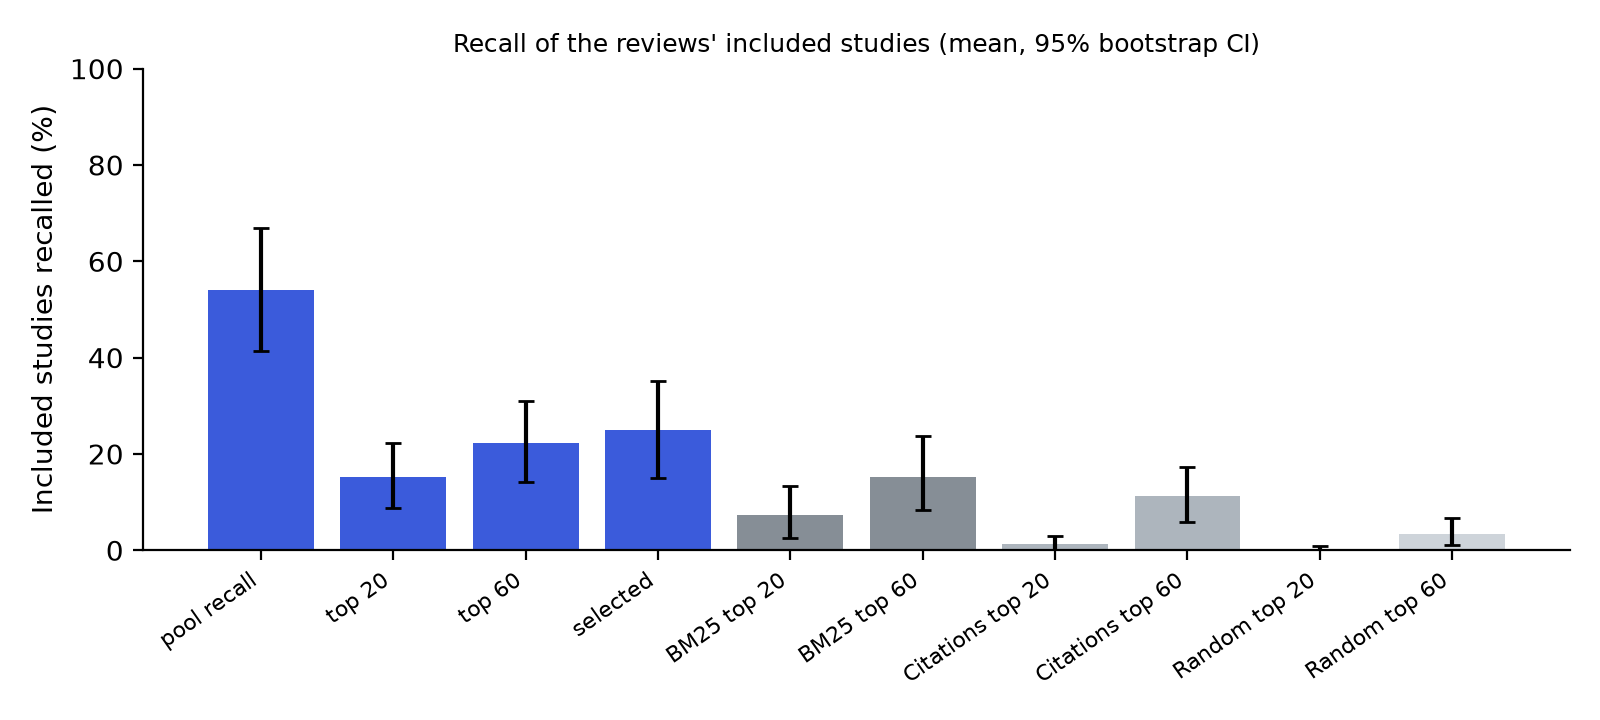
\includegraphics[width=\linewidth]{figures/fig_recall.png}
\caption{Recall of the 22 test reviews' included studies: \tool{}'s candidate pool, the top 20 and top 60 of its
screening order and its selection (blue), and three baselines ranking the same pools (grey). Means with 95\%
bootstrap CIs.}
\label{fig:recall}
\end{figure}

The 100-point score ordered the pools better than each baseline: the top 20 held 15\% of the included studies
against 7\% for BM25 against the question, 1\% for citation count and 0\% at random (top 60: 22\%, 15\%, 11\%, 3\%).
Model screening kept a mean of 87\% of the included studies it saw (median 100\%), with low precision (10\%), as
expected for a step that keeps records unless a criterion is clearly not met. Citation searching and review
reference lists added 15 included studies that no database search returned. The quick-answer mode, which collects
100--170 records per question and selects 20, held 15\% of the reviews' included studies in its pool and 4\% in its
selection: it answers a question quickly but is not a review search.

\subsection{Where included studies were lost}
\label{sec:loss}

Table~\ref{tab:loss} classifies the 538 included studies the systematic-style runs did not select. Eighty per cent
were lost at search. Half of all losses (266) were studies that one of \tool{}'s own PubMed queries matches but that
ranked beyond the 500 records retrieved; one review with 245 included studies accounts for 134 of them. Another 169
were matched by no query. Losses at eligibility (67) and screening (36, of which 27 were eligible but never reached
because of the screening cap and study limit) were smaller.

\begin{table}[t]
\centering
\caption{Where and why the 538 included studies not selected were lost (22 test reviews).}
\label{tab:loss}
\footnotesize
\begin{tabularx}{\linewidth}{>{\raggedright\arraybackslash}Xrr}
\toprule
Stage and reason & Studies & Share \\
\midrule
Search: beyond the retrieval depth (a \tool{} PubMed query matches it) & 266 & 49\% \\
Search: no \tool{} query matches it & 169 & 31\% \\
Eligibility: concept words not matched & 55 & 10\% \\
Screening cap or study limit (eligible, never screened) & 27 & 5\% \\
Eligibility: set aside as a review article by publication type & 10 & 2\% \\
Model screening: a criterion answered ``no'' & 9 & 2\% \\
Eligibility: other (not a research report) & 2 & 0\% \\
\bottomrule
\end{tabularx}
\end{table}

Reading the stored corpora showed three recurring causes. First, selection reads a rule-based parse of the
question so that it does not depend on the model, and where the parse was poor it cost recall: for ``First-line
drugs inhibiting the renin angiotensin system versus other first-line antihypertensive drug classes for
hypertension'', the rules produced the concept ``first-line drugs inhibiting'', and 609 of 640 records were judged
off topic, while the model's plan for the same question named ``renin-angiotensin system inhibitors''. Second, a
question naming a class of interventions (``psychological therapies'', ``inhaled corticosteroids'') was answered by
studies naming its members (cognitive behavioural therapy; fluticasone), which word matching missed when PubMed
mapped the class to a different heading. Third, in 8 of the 9 screening losses the model turned the question's
structure into a required criterion: in ``intralesional treatment versus wide resection'' the comparator became the
criterion ``outcome: wide resection'', and case series of the intervention alone, which the review included, were
screened out.

\subsection{Repeatability and sensitivity}

\emph{Selection given the same records (E2a).} All 44 stored test corpora (22 per mode) reproduced their included
studies, in the same order and with matching content hashes, from their stored records alone, with no network and
no model. Because model screening decisions are stored, this covers the systematic-style selection.

\emph{Model screening of the same records (E2b).} Three repeats of the screening of 1,638 records agreed with each
other on 96--97\% of decisions (Cohen's $\kappa$ 0.91--0.94) and with the original decisions on 90--91\% ($\kappa$
0.80--0.82); the original run screened records in batches in score order and the repeats in sample order, so part
of this difference reflects batch context. Sensitivity on the 117 included studies in the sample was 92\% originally
and 93\% in each repeat. A second model could not be measured: the free models tried were rate-limited upstream.

\emph{Records found (E2c, E2d).} Repeating the searches gave different records: two identical rule-planned repeats
shared a median of 63\% of their records (lowest 24\%), with similar pool recall (34\% and 37\%). The difference came
from sources that did not answer within the time budget in one run, and from citation searching that Semantic
Scholar rate-limited, which adds all or nothing. Model planning raised pool recall from 34--37\% (rules) to 54\%;
re-planning each question three times with the model gave the same concept names (median overlap 1.00) but the
same core PubMed string in only 14 of 66 plans, because the synonyms it adds vary.

\emph{Sensitivity to the score's constants (E3).} Setting each weight or cap to half or one and a half times its value
changed about one of the 20 quick-answer selections (median Jaccard overlap 0.90--0.95) and recall by at most 0.3
percentage points; halving the caps on reviews changed the quick-answer selection most (median overlap 0.57)
without changing recall (Fig.~\ref{fig:sensitivity}). In the systematic-style runs the records the model would
screen were unchanged in most reviews (median overlap 1.00, lowest 0.85).

\begin{figure}[t]
\centering
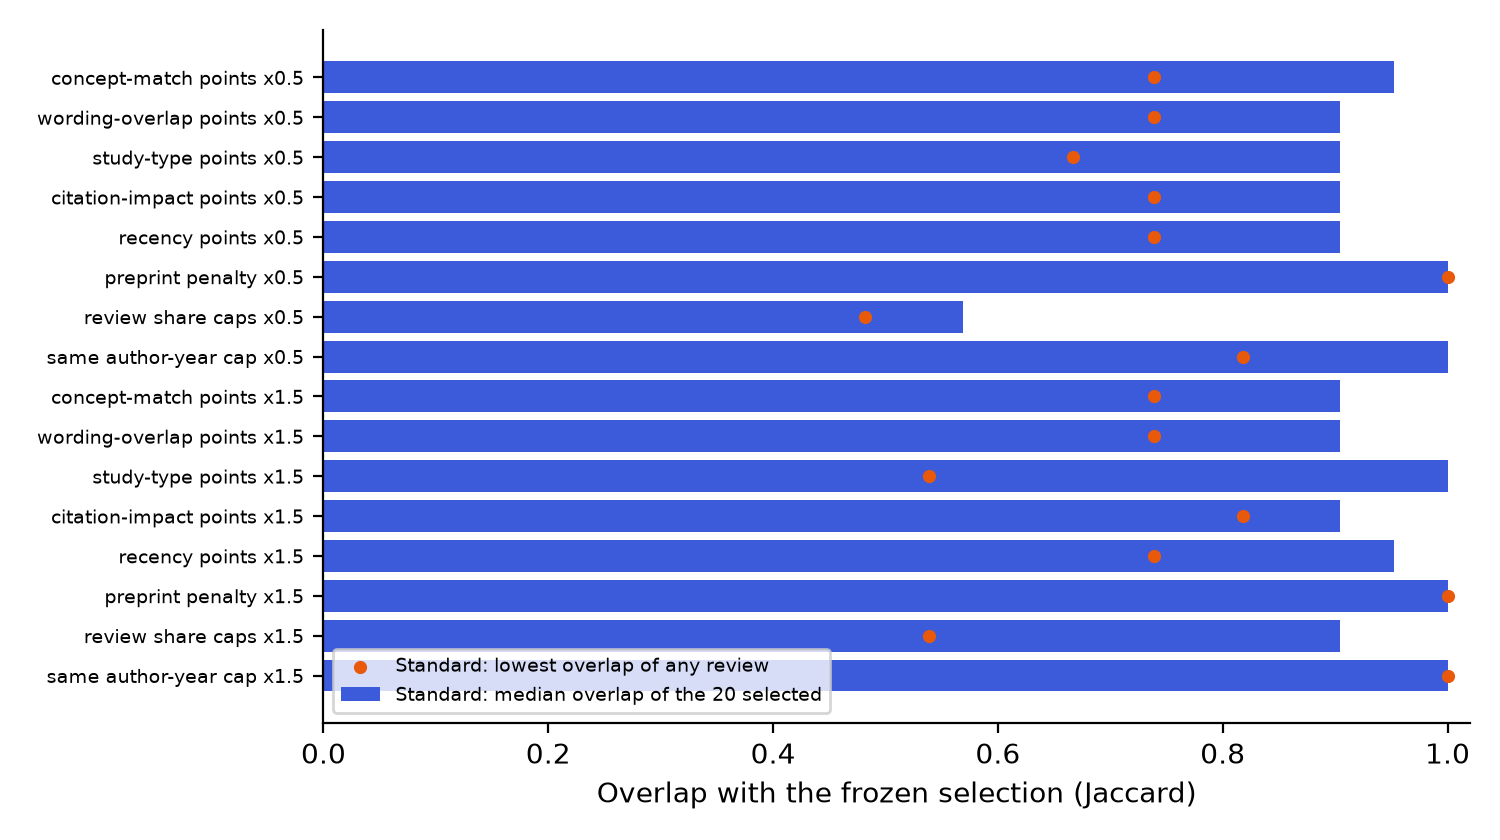
\includegraphics[width=0.85\linewidth]{figures/fig_sensitivity.png}
\caption{Sensitivity of the quick-answer selection to each score weight and cap, set to half and one and a half
times its value: median (bars) and lowest (dots) Jaccard overlap with the frozen selection over the 22 test
reviews.}
\label{fig:sensitivity}
\end{figure}

\subsection{Components and written claims}

\emph{Study type.} With PubMed's publication types removed, the classifier labelled 67\% of 26,114 records
correctly from wording alone; trials had precision 0.88 and recall 0.62, systematic reviews and meta-analyses 0.82
and 0.58, and case reports and narrative reviews were mostly called other primary research. With Semantic Scholar's
own types (2,819 papers) accuracy was 0.78. Because 80\% of the included studies in the test corpora carry PubMed's
own types, which the classifier reads first, these figures apply to the remaining 20\%.

\emph{Duplicate merging.} \PENDING{share of the 100 sampled merges judged to be the same study, by kind of merge}

\emph{Claims in the written synthesis.} Over the 33 model-written analyses, the rule-based checks changed no
narrative and excluded none of 117 structured claims; one narrative needed a corrective retry during generation.
\PENDING{Of the 200 sampled cited sentences, N\% were supported, N\% partly supported and N\% not supported by the
studies they cite (95\% CI); agreement between the two annotators on 50 sentences, Cohen's $\kappa$ = N.}
